\documentclass[12pt, a5paper]{article}
\usepackage[14pt]{extsizes}
\usepackage[utf8]{inputenc}
\usepackage[russian,ukrainian]{babel}
\usepackage{indentfirst}
\usepackage{amsmath,amssymb,amsthm}
\usepackage{mathrsfs}
\renewcommand{\baselinestretch}{1.19}
\renewcommand{\labelenumi}{\theenumi)}
\usepackage{fancyhdr}
 \pagestyle{fancy}
 \fancyhf{}
 \fancyhead[R]{\thepage}
 \fancyheadoffset{0mm}
 \fancyfootoffset{0mm}
  \setlength{\headheight}{17pt}
\renewcommand{\headrulewidth}{0pt}
\renewcommand{\footrulewidth}{0pt}
 \fancypagestyle{plain}{
\fancyhf{}
\rhead{\thepage}}
 \setcounter{page}{1}
\renewcommand{\headrulewidth}{0pt}
%\setcounter{chapter}{0}
%\newtheorem{remark}{Зауваження}[chapter]
%\setcounter{remark}{0}
%\newtheorem{theorem}{Теорема}[chapter]
%\setcounter{theorem}{0}
%\newtheorem{lemma}{Лема}[chapter]
%\setcounter{lemma}{0}
%\newtheorem{result}{Наслідок}[chapter]
%\setcounter{result}{0}
%\newtheorem{definition}{Означення}[chapter]
%\setcounter{definition}{0}
\usepackage{geometry}
\geometry{left=2cm}
\geometry{right=2cm}
\geometry{top=2cm}
\geometry{bottom=2cm}
\usepackage{graphicx}
\usepackage{tikz}  
\usetikzlibrary{graphs}

\begin{document}

\thispagestyle{empty}
\begin{center}
\bigskip
\textbf{\MakeUppercase{Economic Based Integrated Concurrent Fault Tolerant Consensus Algorithm}}
\medskip
\end{center}
\textit{Yevhen Leonchyk, Igor Mazurok, Valeriy Penko}
\\[0.5cm]
\textbf{\large{Annotation}}

\small{This work is devoted to research and develop parallel fault tolerant consensus algorithm for distributed processing systems and information storage with low delays. An essential characteristic of this algorithm is introduction economic model which ensures its sustainable development in accordance with the objectives of functioning. The proposed algorithm was called WWH (What, Where to, How much), because it allows for one pass of the protocol to obtain coordinated decisions on such issues:
\begin{itemize}
\item what information will be storaged;
\item in which place of the synchronized repository it will be written;
\item remuneration of knots for conscientious work.
\end{itemize}

The algorithm is based on the ideas of algorithms SBFT~[1], Raft~[2] and the basic principles of Computable general equilibrium~[3] 
to build the internal economy of the functioning of the system. The algorithm assumes resistance to two types of errors - Byzantine errors and equipment failures.}
\section{Introduction}

The characteristic trend of modern information systems is the transition to a distributive architecture. In this case it is important to provide the following requirements:
\begin{itemize}
\item performance;
\item scalability;
\item tolerance relative to various types of attack;
\item immutable and tampering safety;
\item logic consistency.
\end{itemize}

To support this set of characteristics is used standardized technology which named BlockChain. Due to the distributed nature of these systems the main role plays mechanism of consensus - the ability to make concerted decisions (Wikipedia). In traditional systems based on BlockChain systems is used a consensus like PoW (bitcoin, etherium). However, for many applications this type of consensus is unacceptable because of low system performance (low throughput).

The goal of this work is to develop a version of the consensus protocol that will meet the following requirements:
\begin{itemize}
\item the scale of the system that is typical for corporate tasks (that is, the system presents a high entry threshold to new nodes, and as a result, the number of network nodes is limited to several hundreds);
\item the system must provide a high speed of response to the client request;
\item processing nodes of the system are equal, ensuring its decentralization.
\end{itemize}
\section{Related works}

The most known consensus algorithms are PoW (proof-of-work) and PoS (proof-of-stake), but they are not ideal. For example, a significant disadvantage of PoW is the huge consumption of electricity, which "slows down" the network. To prevent this problem, there is a solution - PoS. However, PoS is not without criticism. Its shortcomings are as follows:
\begin{itemize}
\item PoS gives additional motivation to accumulate funds in the one hands, that can negatively affect the decentralization of the network;
\item If will formed a small group, which collect a lot of money, it can impose its own rules of the network to other participants.
\end{itemize}
Given the above requirements, it is clear that PoS and PoW are not the best solution. Therefore, there is a need to find a suitable consensus algorithm. In this sense, the most discussed in academic publications is the Paxos algorithm~[?]. However, attempts to use it in real systems cause difficulties. Due to this, various modifications of this algorithm have been proposed. In particular, Raft was designed to provide modularity, which in turn led to its clarity and ease of implementation. It contains sufficient means of supporting the information log (ledger) and is focused on the accented use of the leader node and provides only CFT. However, from the point of view of the above requirements, this is not enough, because the system may have Byzantine Fault Tolerance (BFT). Modifications of the Raft algorithm are known, which overcome this limitation~[?]. Some features of these modifications have been used in this work.
\section{Main part}
\subsection{General remarks}

The system consists of nodes communicating over a peer-to-peer protocol. At different stages of the communication protocol, the nodes perform different roles:

\textbf{masterNode} -  node which signs and stores certificates;

\textbf{receptionNode} - node which receives a client CSR (Certificate Signing Request). It also  receives a client payment and performs remuneration for nodes;

\textbf{Leader} -  node which coordinates message exchange between the other masterNodes.

\textbf{Term} -  number of the epoch from the start of network work, where current Leader is operate. The number of the term is increased by one when the Leader changes;

\textbf{Beat} -  the sequence of protocol steps performed from the CSR receiving to the certificate recording in the system BlockChain. 
\subsection{Tokenomica: description, formalization and parameters}

\textbf{Tokenomica} -  set of relations between elements of a distributed system, which is based on using crypto currency (tokens). In our system, the tokenomica is aimed at ensuring high performance of individual components (fault tolerance, integrity, performance). Such indicators of individual components should ensure the stability of the system as a whole.

For searching optimal parameters for the functioning of the system and its components, we define an information model containing information about the chronology of the actions performed by participants in the system of actions.

Such model can be formulated in a natural way on the basis of a representation of the functioning of the system in the form of an oriented loaded graph whose nodes are the servers of the system (more precisely, their participation in a certain stage of interaction in a certain role protocol), communications-messages or queries marked with information accompanying these communications.
\begin{center}
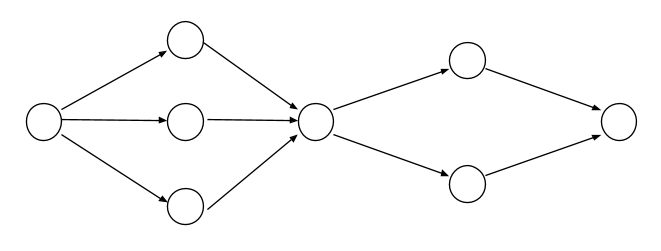
\includegraphics[scale=0.5]{Introduction.png}
\end{center}
A route in such graph describes the sequence of execution of the stages of the communication protocol, which leads to the achievement of the result.

\subsection{The protocol for issuing a certificate including the node’s contribution}

In order to provide sustainable functionality the system has to satisfy the next requirement: the total node number n must be greater than 3f+2c where

f - the maximum number of faulty (byzantine) nodes;

c - the maximum number of crashed nodes (at least within established period of time).

%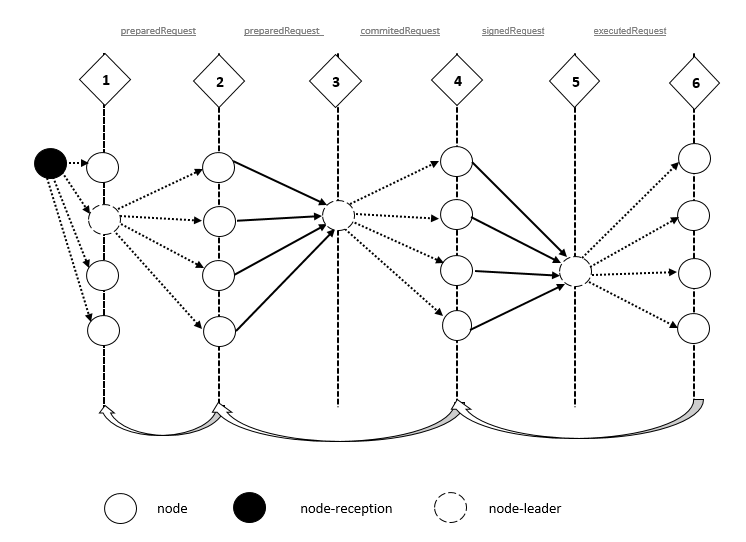
\includegraphics[scale=0.5]{2.png}

\begin{center}
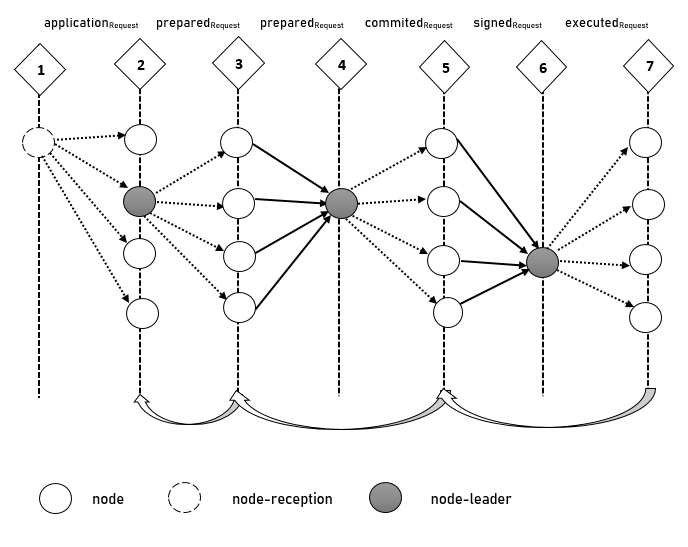
\includegraphics[scale=0.5]{2_2.png}
\end{center}

\subsection{Fault Tolerant Election Protocol}
Information flows of the fault tolerant election protocol are shown in the following figure.

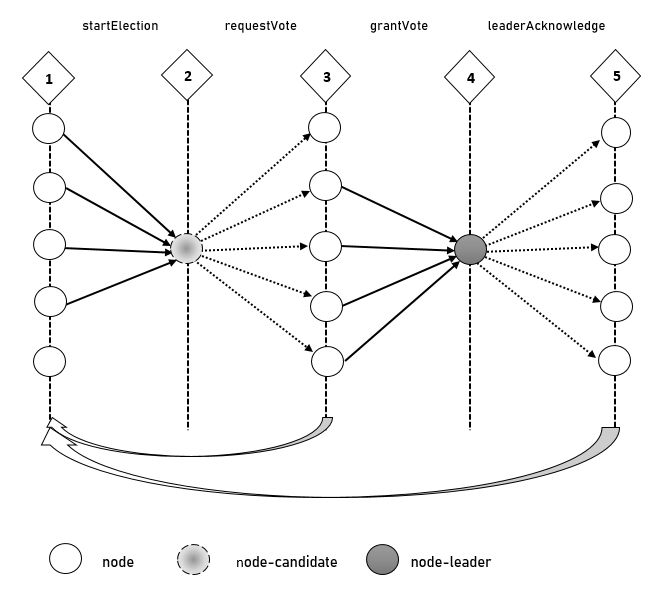
\includegraphics[scale=0.5]{1.png}

Each node maintains in its state an integer value, called a term (t). At the beginning of each leader election procedure, node-candidate increases the value of its term by 1. Thus, the term used as  the conventional discrete time of a distributed system for synchronizing nodes activity. It expresses the number of attempts (not necessarily successful) to re-elect a new leader.

The protocol consists of five steps.

1) A TimeOut event occurs, if for a certain period of time the node does not receive messages from other nodes or receives incorrect data from them. As a result, this node increases its term by 1 and initiates the re-election of the new leader, sending the node with the number t mod n inside the message \textbf{\textit{startElection}} of the following format:

\begin{table}[h!]
\begin{center}
\begin{tabular}{|c|c|c|}
\hline
From &  Message & To \\
\hline
\small{nodе-sender} & \small{T} & \small{node with number $t_{node}mod\; n$}\\
\hline
\end{tabular}
\end{center}
\end{table} 

2) If the node has received a sufficient (2f+1) number of checked \textbf{\textit{startElection}} messages with the same t it becomes the node-candidate for the term t. As a result, it sends a \textbf{\textit{requestVote}} message to all nodes. This message contains the value of term, the last element of its log and 2f+1 \textbf{\textit{startElection}} requests:

\begin{table}[h!]
\begin{center}
\begin{tabular}{|c|c|c|}
\hline
From &  Message & To \\
\hline
\small{nodе-candidate} &\footnotesize{t; lastLogEntry; startElection[2f+1]}& \small{All nodes}\\
\hline
\end{tabular}
\end{center}
\end{table} 

3) Node that receives the requestVote message checks the following condition
$$(t_{requestVote} \ge t_{node})$$
and 
$$(requestVote\; has\; 2f+1\; checked\; startElection\;  messages)$$ 
and 
$$(lastLogEntry_{requestVote}\; corresponds\; lastLogEntry_{node})$$
 
If all checks successful, node gives its vote to the node-candidate by sending it a \textbf{\textit{grantVote}} message of the following format:
\begin{table}[h!]
\begin{center}
\begin{tabular}{|c|c|c|}
\hline
From &  Message & To \\
\hline
\small{nodе-sender} & & \small{node-candidate}\\
\hline
\end{tabular}
\end{center}
\end{table} 

If the above check fails, the node tries to initiate the re-election procedure (step 1-2)

4) If the node-candidate receives 2f+1 valid grantVote messages, it becomes the node-leader and sends to the rest nodes the leaderAcknowledge message certifying the fact of its leadership. This message contains the leader's term and information about the nodes that gave voice to the leader:

\begin{table}[h!]
\begin{center}
\begin{tabular}{|c|c|c|}
\hline
From &  Message & To \\
\hline
\small{nodе-leader} &\footnotesize{t; lastLogEntry; grantVote[2f+1]} & \small{All nodes}\\
\hline
\end{tabular}
\end{center}
\end{table} 

5) The node that receives the message \textbf{\textit{leaderAcknowledge}}, checks it, taking into account the value of term (the term in the message is greater than the term of the node), increases its term and becomes a node-follower (usual node)  using this leader.
If this check fails, the node tries to initiate the re-election procedure (step 1-2)

\subsection{Economics of certificate issuance}

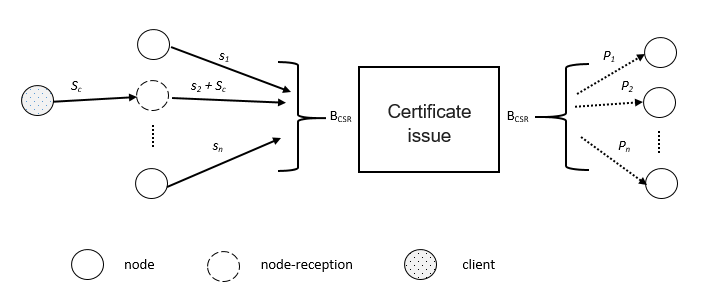
\includegraphics[scale=0.5]{3.png}

\subsubsection{Budgeting}
\subsubsection{Distribution of remuneration}
\subsection{Economy of recording and storage}
\subsubsection{Determination of share}
\subsubsection{Attacks}
\subsection{Charge of remuneration}

To calculate the compensation, we will calculate the contributions and shares of the participants.
\subsubsection{Nodes Contributions}
\subsubsection{The proportion of nodes}
\subsubsection{Node Rewards}
\subsubsection{Timeouts}
\section{Conclusions}

\textbf{\large{Bibliography}}
\small{\begin{enumerate}
\item SBFT: a Scalable Decentralized Trust 
\\
Infrastructure for Blockchains // Distributed, Parallel and Cluster Computing, 2018.
\item Dennis Wang, Nina Tai, Yicheng An. Byzantine Fault Tolerant Raft 
\item Federico Perali, Pasquale Lucio Scandizzo. The New Generation of Computable General Equilibrium Models: Modeling the Economy, - Springer: 2018. - 342 pp.
\end{enumerate}}

\end{document}